\section{Analysis}
\subsection{Limitations}
The algorithm does not solve \textsc{Shortest Odd Path} in the absolute general case, but rather has some limitations. These are: 
\begin{itemize}
    \item The input graph must be undirected, otherwise we cannot use blossoms the way we do.
    \item The edges must have either non-negative weights or no weights at all, otherwise we cannot guarantee that $d^+_u$ and $d^-_u$ are correct when we scan a vertex $u$.
\end{itemize}
\todo{Are there more limitations? Should this section go somewhere else?}

\subsection{Complexity}
In this section we will give a theoretical analysis of our algorithm's running time.

\subsubsection*{Proof of the running time}
Let $(G,s,t)$ be an instance of \textsc{Shortest Odd Path}, let $n := |V|$ and let $m := |E|$. \\
Claim: the algorithm runs in time at most $O(m \cdot \log m)$, or $O(m \cdot \log n)$ of the graph is simple.
\begin{proof}  
    First of all, we construct the mirror graph $H$ with $2n-2 \in O(n)$ vertices and $2m - deg(s) - deg(t) \in O(m)$ edges, in time $O(n+m)$.
    
    With our \pyth{completed} array we can guarantee that each vertex is scanned at most once, and the scanning operation just loops through all the neighbours. Therefore, the total cost of all the scans is $O(n + \sum_{u \in V} deg(u)) = O(n + 2m) = O(n + m)$.

    The blossom operation is a little more complicated. Thanks to the overly complicated code in our \pyth{backtrack_blossom} procedure in Section \ref{subsection:backtracking-blossom-edges}, we can backtrack from a blossom edge and determine the vertices in the blossom in time linear to the size of the blossom. Setting their values for $d^+$ and $d^-$ can also be done in linear time, and the potential scans have already been accounted for above. The key point here is that we shrink the blossom into a psuedonode afterwards: each vertex can then only be part of such a blossom procedure at most once. Even though we may compute many blossom edges, the total amount of work will therefore never exceed $O(n)$.

    Lastly, we have the main loop, which iteratively pop vertices and blossom edges from the queue. Each of the $O(n)$ vertices may be put into the priority queue many times, at most once for each of its neighbours. That is a total of $O(m)$ vertices in the queue, for a total cost of $O(m)$. Though it is unlikely, in the extreme case all edges may be put in the queue as blossom edges as well, again for a total cost of $O(m)$. In total, enqueueing everything costs $O(m)$, and dequeueing everything costs $O(m \cdot \log m)$.

    In total, the algorithm runs in time $O(n+m) + O(n+m) + O(n) + O(m) + O(m \cdot \log m) = O(m \cdot \log m)$.
    If the graph is simple, then we can simplify it further to $O(m \cdot \log n^2) = O(m \cdot 2 \cdot \log n) = O(m \cdot \log n)$.
\end{proof}

\subsubsection*{Running times of other variants}
A running time of $O(m \cdot \log n)$ means that the algorithm generally performs well on sparse graphs. We chose this algorithm with this running time because in \Cref{chapter:network-diversion} we will use it on planar graphs, where $m \leq 3n-6$, as shown in \Cref{corollary:m-leq-3n}.

We should note, however, that there are also other known polynomial algorithms for \textsc{Odd Shortest Path}. In the same paper that Derigs gave the algorithm of this chapter, he also gave another variant \cite{source:derigs_shortest_odd_path}. The main difference is that we drop the priority queues and use a list instead, and in the control loop instead search through the entire list and pop the element with the lowest priority. That search takes time at most $O(n)$, and can be done at most $n$ times, for a total running time of $O(n^2)$. If the input graphs are dense, then this $O(n^2)$ algorithm may be preferable to our $O(m \log n)$ algorithm.

\subsection{Benchmarking}
In this section we will give an empirical analysis of our algorithm's running time.

\subsubsection{Testing different data structures for the Basis}
\label{subsubsection:testing-basis}
As shown and discussed in Section \ref{subsection:basis-code}, we have implemented multiple data structures to keep track of the basis of each vertex. One of them is based on the Observer pattern, the other on the well-known UnionFind structure. We have tested both on 6 different real-life graphs, and we show the results below. We ran our shortest odd path algorithm on each graph 40 times, 20 for each structure, and noted the fastest times for each. The vertices with id's 0 and n-1 were chosen as the source and target to paths for, respectively. \todo{reformat}
\begin{center}
    \begin{tabular}{|l | r | r | r | r | c|} 
     \hline
     Graph & n & m & Observer & UF & Change \\ [0.5ex] 
     \hline\hline
     Oldenburg & 6105 & 7035 & 5.1555 ms & 4.6955 ms & -11.277\%\\ 
     \hline
     San Joaquin County & 18263 & 23874 & 6.7046 ms & 5.7347 ms & -14.212\%\\
     \hline
     Cali Road Network & 21048 & 21693 & 19.280 ms & 19.119 ms & +0.1590\%\\
     \hline
     Musae Github \cite{graph:musae-github} & 37700 & 289003 & 21.375 ms & 19.438 ms & -2.4708\%\\
     \hline
     SF Road Network & 174956 & 223001 & 93.494 ms & 87.570 ms & -6.3364\%\\ [1ex] 
     \hline
     Pokec Social Network \cite{graph:soc-pokec} & 1632804 & 30622565 & 13.225 s & 13.774 s & +4.1543\%\\ [1ex] 
     \hline
    \end{tabular}
\end{center}
\todo{cite the rest of the graphs}

\todo[inline]{Also test on Delaunay graphs}

The results are a little mixed. The UnionFind-based structure spends $4.2\%$ more time on the huge Pokec Social Network graph. However, it also either outperforms or does as well as the Observer-based structure on all the other graphs, at best shaving off $14.2\%$ of the time spent on the San Joaquin County graph. Since the UnionFind-based structure outperforms the Observer-based structure on average, we have chosen to use that one for the remainder of this thesis.

\subsubsection{Running times on Delaunay graphs}
\label{subsubsection:odd-path-delaunay-testing}
Like explained in \Cref{section:delaunay}, we have generated 201 Delaunay graphs of sizes 1000, 2000, 3000 etc. to 200 000. For each graph, we have found a source and target with the highest possible shortest path between them, and run our \textsc{Shortest Odd Path} algorithm. The algorithm gets 10 attempts on each input graph, and we take the median and plot it below.

The theoretical running time is $O(m \log n)$, and we have tried our best to come up with constants to create a running time function that matches our algorithm. Remember that in Delaunay graphs we have that $m \leq 6n$, so we have set $m := 6n$ in this function.

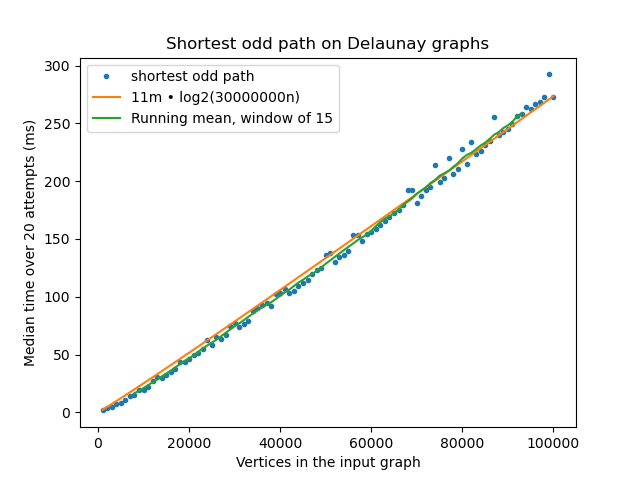
\includegraphics[width=15cm]{figures/bench_plots/shortest odd path.png}

As we can see, the running times grow almost linearly as the inputs grow larger. The slight upwards curve is barely noticable. This is to be expected with a linearithmic theoretical running time.

\subsection{Discussion}
The focus of this thesis is to create an algorithm that performs well on sparse graphs, especially planar graphs, which is why we consider the running times mainly on sparse graphs. If we instead had implemented an algorithm for denser graphs, or just graphs in general, then testing on graphs with more edges would be more appropriate.
\todo{write more here}